\paragraph{Цель работы:} разобраться с программой продольного точения вала.

\subsection*{Команда продольного точения}

Формат команды изображен в таблице \ref{tab:format}. Результат выполнения --- на рисунке \ref{fig:main}.

\begin{longtable}[c]{|c|c|c|c|c|c|c|c|c|}
    \caption{Формат команды}
    \label{tab:format}\\
    \hline
    \multirow{2}{*}{\textbf{G84}} & \textbf{X..} & \textbf{Z..} & \textbf{P0..} & \textbf{P2..} & \textbf{D0..} & \textbf{D2..} & \textbf{D3..} & \textbf{F..}\\
    \cline{2-9}
    \endfirsthead
        & $mm$ & $mm$ & $mm$ & $mm$ & $\mu m$ & $\mu m$ & $\mu m$ & $mm/min$\\
        \hline
\end{longtable}

\begin{figure}[ht]
    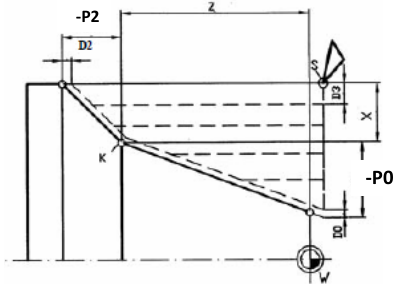
\includegraphics[width=.8\linewidth]{Figures/main.png}
    \caption{Цикл продольного точения}
    \label{fig:main}
\end{figure}

Первая программа использует параметры D0, D2 и D3, тем самым получая форму, изображенную на рисунке \ref{fig:task1}. Вторая программа использует также параметры P0 и P2 (рисунок \ref{fig:task2}).

\subsection*{Первая программа}

\begin{minipage}[t]{.45\textwidth}
    \begin{verbatim}
N0010 G54 G92 X0.000 Z50.000
N0020 G59
N0030 G00 X60.000 Z60.000
N0040 T0101
N0050 G96 S120 F200 M03
N0060 G00 X42.000 Z2.000
N0070 G84 X16.000 Z-30.000
D3=2000 D0=1000 D2=1000
N0080 G00 X60.000 Z60.000
N0090 G53 G56 T0000 M30
    \end{verbatim}
\end{minipage}
\begin{minipage}[t]{.45\textwidth}
    \raggedleft
    Смена системы координат\\
    Инициация смены нуля\\
    Перемещение в точку (60,60)\\
    Выбор первого инструмента\\
    Установка параметров резания\\
    Подход к детали без интерполяции\\
    Установка точки K\\
    Установка параметров\\
    Возврат в начало\\
    Конец программы
\end{minipage}

Здесь S120 --- установка скорости вращения шпинделя, F200 --- скорость подачи, M03 --- вращение шпинделя по часовой стрелке.

G84 --- цикл продольного точения, X и Z задают координаты точки P (рисунок \ref{fig:main}), D3 --- глубину одного прохода, D0 и D2 --- окончательную глубину в осях X и Z соответственно.

\subsection*{Вторая программа}

\begin{minipage}[t]{.45\textwidth}
    \begin{verbatim}
N0010 G54 G92 X0.000 Z50.000
N0020 G59
N0030 G00 X60.000 Z60.000
N0040 T0101
N0050 G96 S120 F200 M04
N0060 G00 X42.000 Z2.000
N0070 G84 X28.000 Z-20.000
D3=2000 D0=1000 D2=1000 P0=-8.000 P2=-5.000
N0080 G00 X60.000 Z60.000
N0090 G53 G56 T0000 M30
    \end{verbatim}
\end{minipage}
\begin{minipage}[t]{.45\textwidth}
    \raggedleft
    Смена системы координат\\
    Инициация смены нуля\\
    Перемещение в точку (60,60)\\
    Выбор первого инструмента\\
    Установка параметров резания\\
    Подход к детали без интерполяции\\
    Установка точки K\\
    .\\
    Возврат в начало\\
    Конец программы
\end{minipage}

Здесь M04 --- вращение шпинделя против часовой стрелки, P0 и P2 задают расстояния по осям X и Z соответственно.

\subsection*{Результат выполнения программ}

\begin{figure}[ht]
\centering
	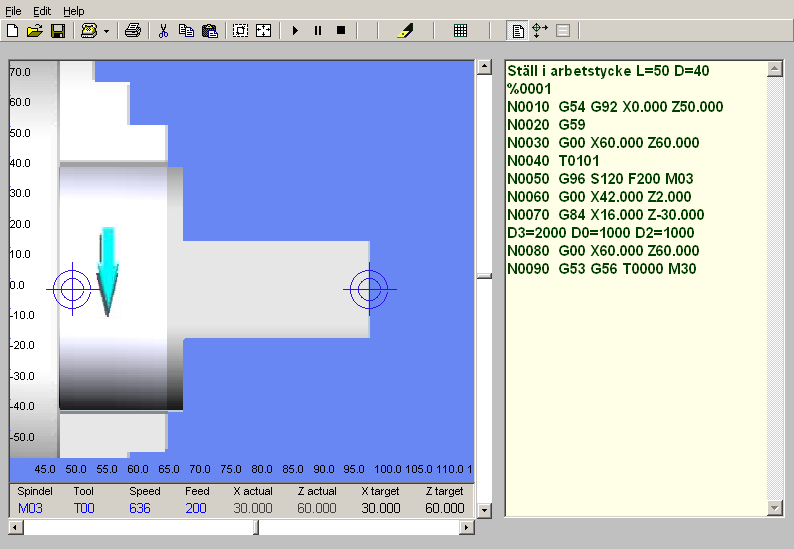
\includegraphics[width=.7\linewidth]{Figures/task1.png}
    \caption{Результат первой программы\label{fig:task1}}
\end{figure}

\begin{figure}[ht]
\centering
	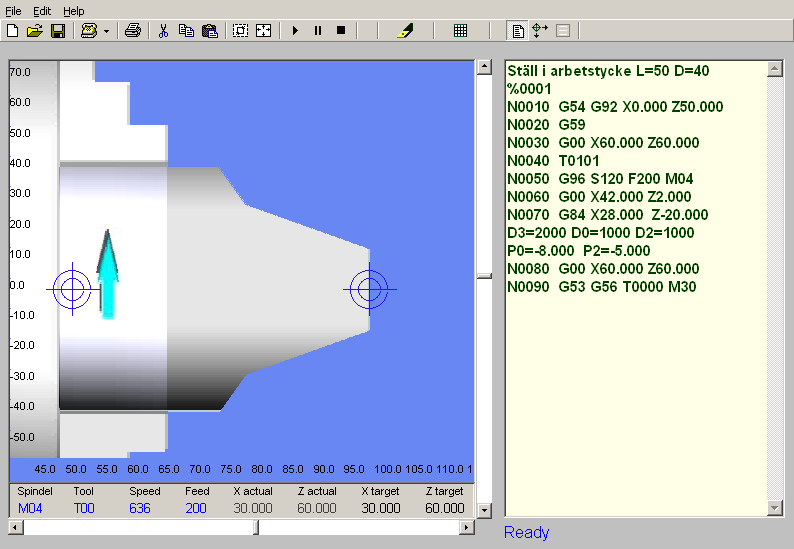
\includegraphics[width=.7\linewidth]{Figures/task2.png}
    \caption{Результат второй программы\label{fig:task2}}
\end{figure}

\subsection*{Выводы}

В лабораторной работе мы изучили цикл продольного точения, выточили две детали определенной формы, узнали за что отвечают параметры директивы G84.

\clearpage
